
\section{Podział projektu}
{W celu zmniejszenia złożoności oraz kosztów utrzymania projektu zdecydowano się na rozbicie architektury na cztery moduły. Każdy z wyodrębnionych modułów ma za zadanie spełniać określoną czynność w architekturze systemu. Rozbicie projektu pozwala  na łatwiejsze zarządzanie kodem oraz, w przypadku dalszego rozwoju przez większą liczbę programistów umożliwia szybkie wdrożenie nowych uczestników projektu. Zastosowanie warstw projektowych bardzo dobrze sprawdza się przy projektach dużej wielkości w przypadkach, gdy programista dąży do rozłożenia odpowiedzialności komponentów w poszczególnych modułach.

W programie w związku z podziałem projektu na pod moduły możemy wyróżnić rozbudowaną architekturę systemu oraz widoczny podział obowiązków poszczególnych pod projektów. W każdym z wydzielonych programów możemy wyróżnić jego odpowiedzialność za pomocą nazw pomocniczych w projekcie tworzonych na podstawie przestrzeni nazw w języku C\#. Zbiór oraz opis wszystkich podprojektów znajduje się w tabeli 4.1.ls }

\begin{table}[htbp]
	\caption{Podział architektury systemu}
	\label{sys-architecture}
	\begin{center}
    \begin{tabular}{ | p{3cm}| p{3cm} | p{6cm} |}
    \hline Nazwa & Typ &  Opis \\ \hline   
    \hline  Moduł aplikacji użytkownika &  Aplikacja \mbox{internetowa} ASP.NET MVC & Aplikacja internetowa odpowiedzialna za sterowanie komunikacji pomiędzy interfejsem użytkownika na stronie internetowej, a logiką aplikacji.\\ \hline
	\hline  Moduł logiki biznesowej & Biblioteka klas & Aplikacja biblioteczna odpowiedzialna za kontrolowanie przepływu informacji pomiędzy aplikacją internetową, do której użytkownik wysyła żądania, a bazą danych na której wykonywane są operacje pobrania danych niezbędnych do stworzenie i wyświetlenia widoku użytkownikowi.\\ \hline
	\hline Moduł  \mbox{bazodanowy} & Biblioteka klas & Aplikacja zawierające modele struktury bazodanowych potrzebnych do stworzenia bazy danych (eng. Code-First)oraz operacji na nich przy użycia języka zapytań funkcyjnych LINQ.\\ \hline
		\hline Moduł testów & Projekt testów jednostkowych & Aplikacja zawierająca scenariusze testowe oraz testy sprawdzające poprawność działania kodu poprzez sprawdzanie oczekiwanego wyjścia z metod.\\ \hline
	\end{tabular}
\end{center}
\end{table}

\section{Wzorce architektoniczne}
{W celu poprawnej integracji modułów skorzystano z wielu wzorców architektonicznych oraz projektowych. Jednym z najpopularniejszych wzorców architektonicznych w aplikacjach internetowych jest wzorzec Model-Widok-Kontroler (eng. Model-View-Controller, MVC) zakładający rozkład podziału obowiązków na trzy główne człony programu. Kontroler we wzorcu pełni funkcję klasy odpowiedzialnej za przyjmowanie żądań użytkownika w celu pobrania strony, danych lub uzyskania dostępu. Jest to część modułu odpowiedzialna za zarządzanie przepływem informacji pomiędzy modelami, a widokami. Kontroler w przypadku aplikacji z tak rozbitą architekturą przekierowuje dane otrzymane od użytkownika do modułu odpowiedzialnego za logikę biznesową. Rezultatem wykonania metod na modułach jest otrzymanie wynikowego modelu bazodanowego, który następnie jest przekazywany do widoku pod postacią Modelu Widoku (eng. ViewModel). Transformacja modelów jest niezbędna ze względu na bardzo dużą ilość danych zwracanych z serwisu, które nie zawsze są potrzebne przy tworzeniu widoku użytkownika oraz możliwość zmniejszenia złożoności operowanego modelu. Dane przekazywane do widoków przy pomocy silnika Razor tworzą stronę w formacie HTML z nałożonymi informacjami zwróconymi z bazy danych.

W wielu aplikacjach internetowych w architekturze Model-Widok-Kontroler programista dąży do uzależnienia nowo utworzonych klas kontrolerów od pewnych, już utworzonych w aplikacji składowych, jakimi są serwisy. Umożliwiają one wydzielenie logiki biznesowej do osobnych klas oraz zmniejsza ilość kodu napisanego w kontrolerze, przez co klasa ta pełni funkcję pośrednika pomiędzy widokiem, a modelem bazodanowym. Niepotrzebne operacje bazodanowe w kontrolerze oraz duża ich złożoność powoduje duże trudności w późniejszym rozwoju aplikacji oraz brak możliwości ponownego użycia kodu. 

Nowo tworzone kontrolery mogą w bardzo szybkim czasie zyskać dużą liczba funkcjonalności dzięki zastosowaniu wzorców architektonicznych Odwróconego sterowania oraz Wstrzykiwaniem zależności. Skorzystanie z nich umożliwia uzyskanie funkcjonalności, w której możemy swobodnie podłączać oraz odłączać kolejne moduły wpływając na zwiększenie lub ograniczenie funkcjonalności w programie. Dobrymi praktykami programisty jest również ponowne używanie raz napisanego kodu w wielu miejscach. Operacje, które są wykonywane na katalogach oraz plikach są do siebie zbliżone, mimo że korzystają z dwóch różnych kontrolerów odpowiedzialnych za przepływ informacji. Kontrolery te mimo innych zastosowań korzystają z tych samych metod napisanych w serwisie logiki biznesowej. Zastosowanie wzorców spowoduje wzbogacenie kontrolera na początku jego istnienia o stworzone wcześniej funkcjonalności, które mogą zostać wykorzystane ponownie, zmniejszając tym samym złożoność kodu oraz ułatwiając późniejszą modyfikację lub rozwój. 

Szczególnie wartym uwagi wzorcem architektury jest Wstrzykiwanie zależności. Kontroler mógł zostać uzależniony od pewnego rodzaju klas przy wykorzystaniu biblioteki Unity, dla języka C\#. Wstrzykiwanie zależności polega na przesyłaniu do konstruktora kontrolera obiektów zdefiniowanych przez programistę w konfiguracji biblioteki. Bez mechanizmu Unity, byłoby to zadanie bardzo ciężkie do zrealizowania, ponieważ klasy pełniące funkcje kontrolerów w aplikacjach internetowych są wywoływane przez użytkownika aplikacji poprzez skierowanie żądania pod odpowiedni adres witryny, zatem nie jesteśmy w stanie przekazać do konstruktora kontrolera parametrów, a jedynie do wywoływanej metody, nazywanej akcją. Aby móc wstrzyknąć złożoną strukturę danych jako parametr metod inicjalizujących należy przygotować interfejs określający funkcjonalność przesyłanego modelu oraz powiadomić bibliotekę Unity w konfiguracji o możliwości wstrzykiwania podanego typu danych do kontrolera. Operacja w bardzo wielu miejscach zmniejsza złożoność kodu. Rozwiązanie może dla programistów nie zaznajomionym z wzorcem Wstrzykiwania zależności sprawić wiele problemów w przypadku dodawania funkcjonalności do kontrolera uzależnionego od pewnych struktur danych.

Ostatnim wzorcem architektonicznym użytym w projekcie jest Odwrócone sterowanie. Bardzo częstym błędem programistów tworzących aplikacje internetowe jest pisanie zaawansowanej oraz złożonej logiki w klasach kontrolera. Kod napisany w akcji jest nie możliwy do ponownego użycia w innych miejscach aplikacji, ponieważ nie zalecane jest tworzenie obiektów kontrolerów w innych kontrolerach. Ponadto kontroler pełni funkcję pośredniczącą pomiędzy logiką bazodanową, a użytkownikiem, w związku z tym tworzenie złożonych operacji na danych w akcjach w znacznym stopniu naruszają dobre praktyki przyjęte przy pisaniu kontrolerów. Stosowanym podejściem w takich sytuacjach jest wydzielanie logiki do osobnych klas odpowiedzialnych za przepływ informacji. W przypadku złożonych aplikacji internetowych zalecane jest wydzielenie klas odpowiedzialnych za przetwarzanie danych do osobnych projektów. Rozwiązanie te powoduje łatwiejszą orientację w kodzie oraz utrzymuje porządek w strukturze projektowej.
}

\section{Przepływ danych}

{W celu komunikacji pomiędzy użytkownikiem,a bazą danych, klasy pełniące funkcję kontrolerów przekazują odebrane oraz sprawdzone, pod względem poprawności danych, modele do serwisów wzorca Odwrotnego sterowania. Cała logika działania aplikacji oraz sposób wykonywanych operacji znajduje się w klasach pełniących funkcję serwisów.
 Każda ze struktur danych musi zostać zaimplementowana na podstawie wcześniej utworzonego interfejsu, który jest wymagany przez mechanizmy Wstrzykiwania zależności. Struktury serwisów używają generycznych repozytoriów w celu dostępu do danych znajdujących się w bazie danych. 
 
 Każde z repozytoriów inicjalizowane jest w serwisie w momencie potrzeby wykonania operacji bazodanowej na bazie danych. Interfejs, na podstawie którego został stworzony komponent umożliwia podstawowe operacje na bazie danych takie jak: tworzenie, czytanie, aktualizacje oraz usuwanie obiektów. Implementacja repozytorium umożliwia wykonanie wymienionych czynności na dowolnym obiekcie bazodanowym. Raz utworzony obiekt, istnieje przez cały okres czasu potrzebnego na przetwarzanie żądania użytkownika. W przypadku potrzeby implementacji dodatkowych funkcji do generycznego repozytorium dodanie ewentualnego kodu do klasy skutkowałoby rozszerzeniem wszystkich pozostałych repozytoriów. W związku z tym zastosowano mechanizm metod rozszerzonych dla określonego typu klasy odpowiedzialnej za komunikację z bazą danych. }
\\
\begin{center}
	\makebox[\textwidth]{	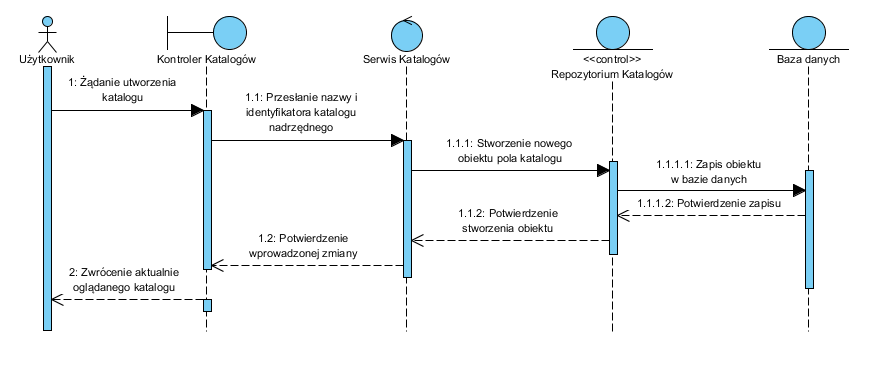
\includegraphics[width=\paperwidth]{obrazy/4.3 przeplyw danych}}
	\captionof{figure}{Diagram sekwencji tworzenia katalogu}

\end{center}

\section{Komunikacja z chmurą danych Azure}
{
Aplikacja w celu przechowywania przesyłanych przez użytkownika plików potrzebuje przestrzeni dyskowej, na której dane mogłyby zostać zapisane. Zarządzanie plikami na serwerze może powodować dużą liczbę problemów między innymi z dostępami do plików oraz katalogów na maszynach, na których aplikacja działałaby bez uprawnień administratorskich. Alternatywnym rozwiązaniem jest magazynu danych oferowany przez usługodawców rozwiązań chmurowych. W celu implementacji przechowywania danych na serwerze skorzystano z chmury Azure z usługi konta magazynu. Wszystkie dane przesłane przez użytkownika zostają zapisane w koncie magazynowym w kontenerze właściciela przestrzeni. Chmura Azure umożliwia podstawowe operacje do zarządzania danymi takie jak dodawanie, usuwanie oraz pobieranie danych. Informacje na temat przechowywanych plików w magazynie znajdują się w bazie danych aplikacji.
}